\chapter*{Proposition 16}
\label{prop:16}

\begin{figure*}[ht]
    \begin{center}
    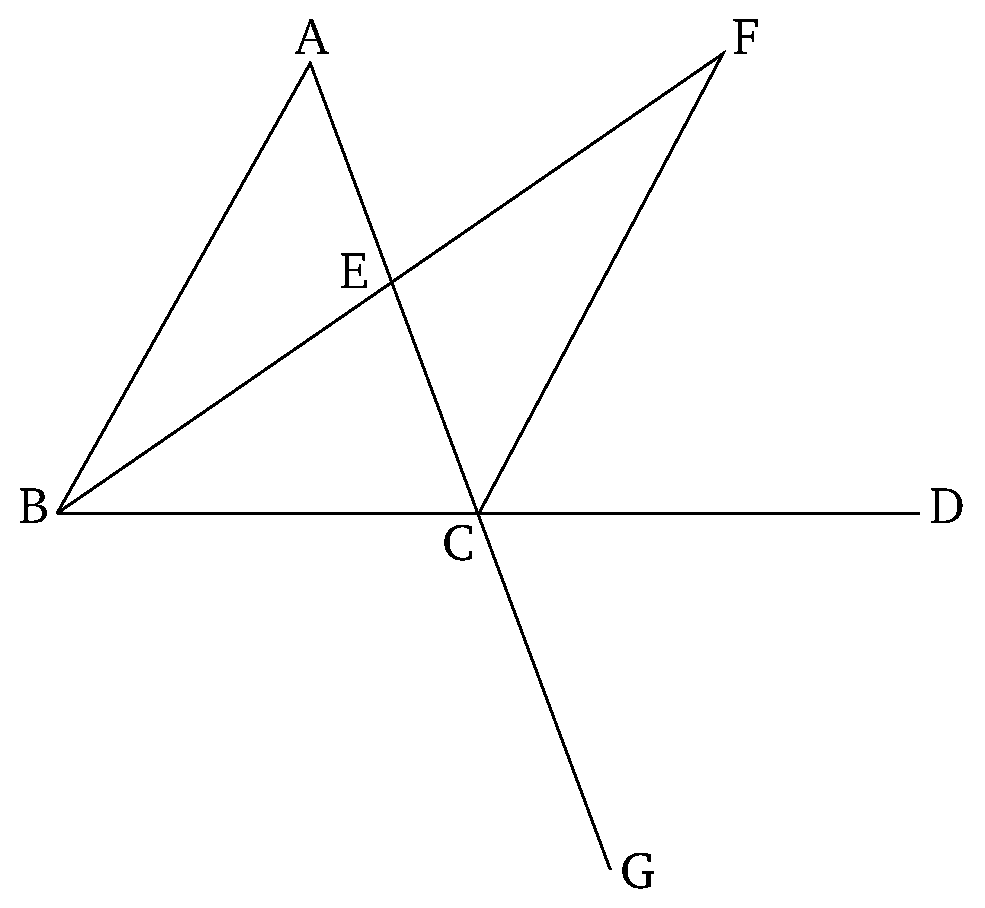
\includegraphics[width=0.5\linewidth]{figures/fig16e.eps}
    \label{fig:prop_16}
    \end{center}
\end{figure*}

For any triangle, when one of the sides is produced, the external angle
is greater than each of the internal and opposite angles.

Let $ABC$ be a triangle, and let one of its sides $BC$ have been produced 
 to $D$. I say that the external angle $ACD$ is greater than each of the
 internal and opposite angles, $CBA$ and $BAC$.
 
Let the (straight-line) $AC$ have been cut in half at (point) $E$ [Prop.~1.10].
 And $BE$ being joined, let it have been produced in a straight-line to
 (point) $F$. And let $EF$ be made equal to $BE$ [Prop.~1.3], and let $FC$ have been joined, and let $AC$ have been drawn through to (point) $G$.

Therefore, since $AE$ is equal to $EC$, and $BE$ to $EF$, the two (straight-lines)
 $AE$, $EB$ are equal to the two (straight-lines) $CE$, $EF$, respectively. 
 Also, angle $AEB$ is equal to angle $FEC$, for (they are)
 vertically opposite [Prop.~1.15]. Thus, the base $AB$ is equal to the base
 $FC$, and the triangle $ABE$ is equal to the triangle $FEC$, and the remaining
 angles subtended by the equal sides are equal to the corresponding remaining angles [Prop.~1.4]. Thus, $BAE$ is equal to $ECF$. But $ECD$ is greater than $ECF$. Thus,
 $ACD$ is greater than $BAE$. Similarly, by having cut $BC$ in half,  it can  be shown (that) $BCG$---that is to say, $ACD$---(is) also greater than $ABC$.
 
Thus, for any triangle, when one of the sides is produced, the external angle
is greater than each of the internal and opposite angles. (Which is) the very thing
it was required to show.


\section*{Commentary}

\begin{proposition}\label{proposition_16}\lean{Elements.Book1.proposition_16}\leanok
    $BC$ is an edge of $\triangle~ABC$ and is extended to $D$. Then, we have $\angle~ACD~>~\angle~CBA$ and $\angle~ACD~>~\angle~BAC$.
\end{proposition}
\begin{proof}
    \uses{proposition_3,proposition_4,proposition_10,proposition_15}\leanok
    Euclid only proved $\angle~ACD~>~\angle~CBA$, though the proof of $\angle~ACD~>~\angle~BAC$ is almost identical.
\end{proof}
